\section{A deterministic inverse and a Brownian sampler}
\label{sec:decoder}

The response estimate permits us to reconstruct the observations from their
innovations.  We first prove the deterministic statement on the full product
path space.  For a countable set $I$, write
\[
 \mathcal C_I=\prod_{i\in I}C([0,\infty),\R),
\]
with the product of the compact-open topologies and its Borel sigma-field.
For $z\in\mathcal C_I$, let $z(t)=(z_i(t))_{i\in I}$.

\begin{lemma}[Deterministic inversion]\label{lem:inverse}
Let $b:[0,\infty)\times\R^I\longrightarrow[0,1]^I$ be jointly Borel.
Suppose that a constant $0\le L<\infty$ satisfies
\begin{equation}\label{eq:abstract-lipschitz}
 \sup_{i\in I}|b_i(t,y)-b_i(t,y')|
 \le L\sup_{j\in I}|y_j-y'_j|
\end{equation}
for every $t\ge0$ and every $y,y'\in\R^I$ whose coordinate differences
have finite supremum.  Then, for every $w\in\mathcal C_I$, there is a
unique $Z(w)\in\mathcal C_I$ satisfying
\begin{equation}\label{eq:inverse-equation}
 Z_i(w)(t)=w_i(t)+\int_0^t b_i(s,Z(w)(s))\,ds,
 \qquad i\in I,\quad t\ge0.
\end{equation}
The map $Z:\mathcal C_I\longrightarrow\mathcal C_I$ is Borel and
causal: its restriction to $[0,T]$ depends only on the input restricted
to $[0,T]$.  It commutes with every coordinate relabeling under which
the drift is equivariant.
\end{lemma}

\begin{proof}
All integrals below are ordinary scalar Lebesgue integrals.  Define
\begin{equation}\label{eq:picard}
 Z^0(w)=w,\qquad
 Z_i^{k+1}(w)(t)
 =w_i(t)+\int_0^t b_i(s,Z^k(w)(s))\,ds,
 \qquad k\ge0.
\end{equation}
These iterates are defined for every input and have continuous coordinates.
Indeed, a continuous coordinate path family gives a Borel map into
$\R^I$, so the integrand is Borel and bounded; its indefinite integral
is continuous.  The initial increment is bounded by $t$, uniformly in
$i$.  Induction using \eqref{eq:abstract-lipschitz} gives
\begin{equation}\label{eq:picard-bound}
 \sup_{i\in I}|Z_i^{k+1}(w)(t)-Z_i^k(w)(t)|
 \le \frac{L^k t^{k+1}}{(k+1)!},\qquad k\ge0,
\end{equation}
where $L^0=1$, including when $L=0$.  At the induction step the
differences of the two input fields are bounded by the preceding
estimate, so the hypothesis of \eqref{eq:abstract-lipschitz} applies.

For every finite $T$, the bounds in \eqref{eq:picard-bound}, with $t$
replaced by $T$, have finite sum.  Thus the iterates converge to a limit
$Z(w)$ uniformly over all coordinates and all $t\in[0,T]$ in the sense
that
\[
 \sup_{i\in I}\sup_{0\le t\le T}
 |Z_i(w)(t)-Z_i^k(w)(t)|\longrightarrow0.
\]
Each coordinate of the limit is continuous.  The Lipschitz estimate
then gives uniform convergence of the corresponding drifts on
$[0,T]$, allowing passage through each integral in \eqref{eq:picard}.
This proves \eqref{eq:inverse-equation}.
The uniform estimates concern differences from the same input: the
input itself may be unbounded over $I$, and its coordinates may have
no common modulus of continuity.

For any other solution $z$, boundedness of $b$ gives
$\sup_i|z_i(t)-w_i(t)|\le t$.  Repeating the same induction
yields
\[
 \sup_{i\in I}|z_i(t)-Z_i^k(w)(t)|
 \le \frac{L^k t^{k+1}}{(k+1)!}.
\]
Letting $k\to\infty$ proves uniqueness for every input.

We next verify measurability on this entire path space.  The evaluation
map $(s,z)\mapsto z(s)$ from $[0,\infty)\times\mathcal C_I$ to
$\R^I$ is continuous.  If $Z^k$ is Borel, the integrand
$(s,w)\mapsto b_i(s,Z^k(w)(s))$ is jointly Borel.  Parameterized
integration of a bounded Borel function shows that its integral from
$0$ to $t$ is Borel in $(t,w)$.  Consequently every rational-time
coordinate evaluation of $Z^{k+1}$ is Borel.  Such evaluations
generate the Borel sigma-field of $\mathcal C_I$, proving inductively
that every $Z^k$ is Borel.  Their limits at rational times prove that
$Z$ is Borel as well.

Finally, the iteration uses only times up to its time argument, which
proves causality.  A coordinate relabeling that intertwines the drifts
also intertwines each step of \eqref{eq:picard} and hence its limit.
This applies equally to a bijection between two different countable
index sets with corresponding drifts.
\end{proof}

Here is the sampling consequence in a form that isolates the role of
the response estimate.

\begin{proposition}[Sampling from independent Brownian paths]
\label{prop:brownian-sampler}
Let $\nu$ be a probability law on $\{0,1\}^I$, where $I$ is countable,
and for each $i$ choose finite sets $S_n(i)$ increasing to $I$.
Interpret the finite-tilt functions \eqref{eq:finite-tilt} and the
limsup drift \eqref{eq:drift} with this law and these sets.
Suppose that the finite-tilt functions $b_{i,S_n(i)}(t,\cdot)$ are
$L$-Lipschitz in the supremum norm on their finite fields, with one
constant $0\le L<\infty$ for all $i,n$ and $t\ge0$.
Then the drift has the Borel solution map of Lemma~\ref{lem:inverse},
and the Borel map $\Psi:\mathcal C_I\longrightarrow\{0,1\}^I$
defined by
\begin{equation}\label{eq:readout}
 \Psi_i(w)=
 \1\left\{\limsup_{n\to\infty}\frac{Z_i(w)(n)}{n}>\frac12\right\}
\end{equation}
sends the law of independent standard Brownian paths to $\nu$.
The map $\Psi$ inherits every coordinate relabeling equivariance of
the drift.
\end{proposition}

\begin{proof}
Each finite tilt is a ratio of finite sums with a strictly positive
denominator, and is therefore jointly Borel in time and the field.
Its limsup is jointly Borel and takes values in $[0,1]$.
If $d=\sup_j|y_j-y'_j|<\infty$, the assumed response bound gives
\[
 |b_{i,S_n(i)}(t,y)-b_{i,S_n(i)}(t,y')|\le Ld
\]
for every $i,n,t$.  Taking limsups in both directions proves
\eqref{eq:abstract-lipschitz}.  Lemma~\ref{lem:inverse} therefore
applies.  Formula~\eqref{eq:readout} is a Borel predicate on every
input, including those on which the displayed slopes do not converge.

To identify its full output law, use the reference observation model:
take $X\sim\nu$, independently take standard Brownian paths $(B_i)$,
and put $Y_i(t)=tX_i+B_i(t)$.  Lemma~\ref{lem:posterior} identifies
the drift with the posterior mean at each fixed time, and
Lemma~\ref{lem:innovation} shows that
\[
 \widehat W_i(t)=Y_i(t)-\int_0^t b_i(s,Y(s))\,ds
\]
has the law of independent standard Brownian paths.
By this definition, the identity
\[
 Y_i(t)=\widehat W_i(t)+\int_0^t b_i(s,Y(s))\,ds
\]
holds for all $i$ and all $t$ on every realization of the continuous
paths.  It does not require the fixed-time posterior identities to
hold on one event simultaneously at every time.
Deterministic uniqueness in Lemma~\ref{lem:inverse} consequently gives
$Y=Z(\widehat W)$ as path families.  Since $Z$ is Borel, it follows
that independent Brownian input $w$ produces the complete joint path
law of $Y$ under $Z$.

For each $i\in I$ and $\delta>0$, the Gaussian tail bound gives
\[
 \P\bigl(|B_i(n)|>\delta n\bigr)
 \le 2\exp(-\delta^2n/2),\qquad n\ge1.
\]
These probabilities are summable.  Borel--Cantelli and a countable
intersection over $i$ and positive rational $\delta$ give
$B_i(n)/n\to0$ for every $i$ simultaneously, almost surely.
Hence $Y_i(n)/n\to X_i$ simultaneously, and
$\Psi(\widehat W)=X$ almost surely.  This identifies the entire
configuration law of $\Psi(w)$ as $\nu$.  Equivariance follows from
Lemma~\ref{lem:inverse} and the coordinatewise formula
\eqref{eq:readout}.
\end{proof}

Figure~\ref{fig:law-transfer} separates the reference coupling used in the
proof from the sampler driven by fresh independent noise. The same Borel
maps are applied in both rows; the target sample is needed only in the
reference argument.

\begin{figure}[htbp]
\centering
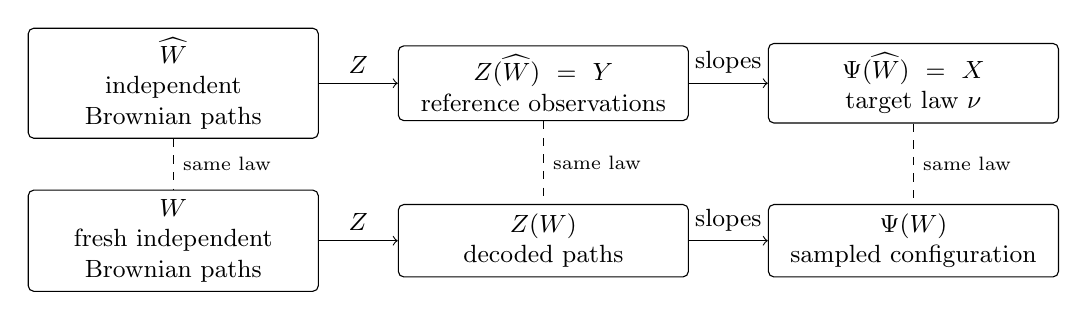
\begin{tikzpicture}[box/.style={draw,rounded corners=2pt,align=center,
  minimum height=0.85cm,text width=3.45cm},font=\small]
\node[box] (a) at (0,0) {$\widehat W$\\independent Brownian paths};
\node[box] (b) at (4.7,0) {$Z(\widehat W)=Y$\\reference observations};
\node[box] (c) at (9.4,0) {$\Psi(\widehat W)=X$\\target law $\nu$};
\node[box] (d) at (0,-2) {$W$\\fresh independent Brownian paths};
\node[box] (e) at (4.7,-2) {$Z(W)$\\decoded paths};
\node[box] (f) at (9.4,-2) {$\Psi(W)$\\sampled configuration};
\draw[->] (a) -- node[above] {$Z$} (b);
\draw[->] (b) -- node[above] {slopes} (c);
\draw[->] (d) -- node[above] {$Z$} (e);
\draw[->] (e) -- node[above] {slopes} (f);
\draw[dashed] (a) -- node[right,font=\scriptsize] {same law} (d);
\draw[dashed] (b) -- node[right,font=\scriptsize] {same law} (e);
\draw[dashed] (c) -- node[right,font=\scriptsize] {same law} (f);
\end{tikzpicture}
\caption{Law transfer in Proposition~\ref{prop:brownian-sampler}.
The upper row is the reference coupling. Deterministic inversion identifies
its middle term pathwise; integer-time slopes recover its right term almost
surely. The lower row uses only independent input paths. Borel measurability
transfers the full joint laws, not only the individual coordinate marginals.}
\label{fig:law-transfer}
\end{figure}

\begin{remark}[The uniformity hypothesis is substantive]
Let $I$ be countably infinite and let $\nu$ assign probability $1/2$ to
each of the all-zero and all-one configurations. For nonempty finite $S$,
all its finite-tilt means are
\[
 b_{i,S}(t,y)=\frac{\exp(a)}{1+\exp(a)},
 \qquad a=\sum_{j\in S}(y_j-t/2).
\]
At $a=0$, the absolute row sum of its field derivatives is $|S|/4$.
Thus no fixed $L$ works along an exhaustion of $I$. The innovation lemma
still applies to this law, but it alone gives no deterministic inverse:
Proposition~\ref{prop:brownian-sampler} uses the uniform response assumption
precisely at that step. Likewise, equivariance of the sampler is asserted
only for relabelings intertwining the chosen drift; arbitrary exhausting
sets need not preserve every symmetry of $\nu$.
\end{remark}

For $\nu=\FUSF_G$, the response bound \eqref{eq:finite-response}
provides the hypothesis of Proposition~\ref{prop:brownian-sampler}
with $L=1/2$.  It remains to obtain the Brownian inputs from the vertex
labels and to verify that the resulting construction is one Borel
rule across graphs.
